\documentclass[11pt,a4paper]{article}
\usepackage[T1]{fontenc}
\usepackage[utf8]{inputenc}
\usepackage{lmodern}
\usepackage[margin=1.85cm]{geometry}
\usepackage{amsmath,amssymb,amsthm,mathtools}
\usepackage{booktabs}
\usepackage{array}
\usepackage{graphicx}
\usepackage{microtype}
\usepackage{xcolor}
\usepackage{hyperref}

\hypersetup{
    colorlinks=true,
    linkcolor=blue!70!black,
    citecolor=blue!70!black,
    urlcolor=blue!70!black
}
\emergencystretch=2.5em

\renewcommand{\abstractname}{Összefoglaló}
\renewcommand{\refname}{Hivatkozások}
\makeatletter
\renewcommand{\fnum@figure}{\thefigure.~ábra}
\renewcommand{\fnum@table}{\thetable.~táblázat}
\makeatother

\title{\textbf{A 4-szimplex $\mathrm{Spin}(10)$ részecskegenezise, 16 paraméteres Paritás--Hermitikus íz-zárása, 5-ös dimenziós protonbomlása és a 24-cellás királis rács szimmetrikus tömeggenerálása}}

\author{Olcsák József\\[0.25em]
\small Független kutató $\cdot$ ORCID: \href{https://orcid.org/0009-0003-7311-6522}{0009-0003-7311-6522}\\
\small Tau Core Kutatási Program --- Paper 30 (\texttt{v1.0.0})}
\date{2026.\ november 24.}

\begin{document}
\maketitle

\begin{abstract}
Önálló, egyetlen paranccsal (\texttt{python3 -W error}, \texttt{rc = 0}) igazolt négypilléres vizsgálatot mutatunk be a Tau Core 4-szimplex ($\sigma_4$, öt határtetraéder $\partial\sigma_4$) és 24-cellás ($D_4/F_4$, bináris tetraéderes csoport $2T$) architektúrájának részecskefizikai, íz-, elektrogyenge hierarchia- és királis rács-szektoraira.
Elsőként a 32 dimenziós $\mathcal{H}_{\partial\sigma_4} = \Lambda^\bullet(\mathbb{C}^5)$ Clifford-térben egzaktul megszerkesztjük a Standard Modell mind a 16 királis állapotát ($\mathbf{16} = \Lambda^{\mathrm{even}}(\mathbb{C}^5)$), mind a 45 $\mathrm{Spin}(10)$ mértékbozont ($12+9+24$), a pontos töltéskvantálást ($Q \equiv N_4 - \frac{1}{3}(N_1+N_2+N_3)$, proton--elektron semlegesség $2{,}22\times 10^{-16}$), a Pati--Salam fa-szintű protonstabilitást és mindhárom Higgs-Yukawa operátort ($\mathbf{10}_H$, $\overline{\mathbf{126}}_H$, valamint a szigorúan antiszimmetrikus 3-gammás $\mathbf{120}_H$, hiba $1{,}11\times 10^{-16}$). Bizonyítjuk továbbá, hogy $|\lambda| = 1/4$ közös egzakt transzfermátrix-sajátértéke a 4-szimplex $K_5$ (multiplicitás 4) és a 24-cellás $P_{24} = A_{24}/8$ (multiplicitás 8) gráfnak ($\cos\theta_{\sigma_4} = 1/4$), és levezetjük a $\mathbb{Z}_6 \subset 2T$ textúra-zérusait.
Másodikként feltérképezzük a 3-generációs íz-elmélet No-Go térképét mind a 18 SM + neutrínó megfigyelhetőn, és azonosítunk egy prediktív, \textbf{16 paraméteres Paritás--Hermitikus zárást} ($\mathrm{PH16}_{a13,h23}$, $\mathrm{dof} = 2$) komplementer 1-gamma vs.\ 3-gamma keveredéssel ($a_{13} = h_{23} = 0$) és egzakt fa-szintű Strong-CP eltűnéssel ($\bar\theta_{\mathrm{QCD,tree}} \equiv 0$, $\det(M_u M_d) > 0$). Ez nem-SUSY $\mathrm{Spin}(10)$-ben $\chi^2 = 0{,}0297$ ($\max|\mathrm{pull}| = 0{,}13\sigma$, $\max|Y| = 0{,}249$), tiszta 1-hurkos MSSM-ben ($\tan\beta = 50$, $\Delta_b = 0$) pedig $\chi^2 = 1{,}3478$ ($\max|\mathrm{pull}| = 1{,}00\sigma$, $\max|Y| = 0{,}534$) eredményt ad.
Harmadikként teljes körű 4D perturbatív No-Go tételeket bizonyítunk a konform Higgs-portál ($\Delta_{\mathrm{FT}} = 3{,}1\times 10^{17}$), a relaxion ($M_{\max} = 3{,}22\times 10^{10}\;\mathrm{GeV} < M_{\mathrm{PS}}$), a $\mathbf{10}\otimes\mathbf{10}$ összetett Higgs-dublett ($0$ színszinglet dublett), a 9 csoportos teljes-$\mathrm{Spin}(10)$ részleges kompozitosság ($0/15$ túlélő), valamint a naiv, kioltás nélküli TeV-SUSY 5-ös dimenziós protonbomlás ($\tau(p\to K^+\bar\nu_\tau) = 3{,}81\times 10^{27}\;\text{év} \ll 5{,}9\times 10^{33}\;\text{év}$ Super-K) ellen. A $\mathrm{PH16}_{a13,h23}$ modellt a Dimopoulos--Wilczek hiányzó-VEV szétválasztással párosítva az extra dublett tömege egyértelműen rögzül $M' = 2{,}64\times 10^{14}\;\mathrm{GeV}$-nél ($\Delta\alpha_3^{-1} = 0$, $M_U = 1{,}04\times 10^{16}\;\mathrm{GeV}$, $39{,}25\times$ triplett-elnyomás), amivel a Mini-Split szkvarok $M_{\tilde q} \in [12{,}0;\; 18{,}4]\;\mathrm{TeV}$ ($\Delta_{\mathrm{FT}} = 3{,}47\times 10^4$) tartománya pontosan a Hyper-Kamiokande 10 éves felfedezési ablakába esik.
Negyedikként bizonyítjuk a 4D 24-cellás rács egzakt $72 = 36(+) + 36(-)$ naiv fermion-kettőződését, igazoljuk a Ginsparg--Wilson Overlap ($2{,}78\times 10^{-16}$) és 5D Domain-Wall határfelületi zérusmódusokat ($1{,}14\times 10^{-5}$ szivárgás), megszerkesztjük az egzakt $\mathrm{Spin}(7)$- és 45-generátoros $\mathrm{Spin}(10)$-invariáns 4-fermionos kölcsönhatásokat, és egzaktul megoldjuk a csatolt 1+1D $\mathrm{Spin}(7)$ Szimmetrikus Tömeggenerálás (SMG) láncot $L=3$-ig ($\dim = 4096$), éles résmentes--SMG kvantum fázisátalakulást mutatva ki $g_c \approx 0{,}20\text{--}0{,}22$-nél szigorúan zérus bilineáris szimmetriasértéssel ($\le 1{,}54\times 10^{-14}$).
\end{abstract}

\paragraph{Publikációs audit: feltételezések, állításhatárok és nyitott kapuk.}
Szigorú négyszintű episztemikus besorolást alkalmazunk (\texttt{PROVEN}, \texttt{PROVEN NO-GO}, \texttt{CONDITIONAL}, \texttt{OPEN}). Minden véges dimenziós Clifford-, mértékalgebra-, transzfermátrix-, 1-/2-hurkos RG-, 9-csoportos bétavizsgálat-, 4D rácsdiszperzió- és $L \le 3$ egzakt sokrészecskés állítást determinisztikusan igazol a \texttt{scripts/build\_paper30\_verification\_and\_figures.py} szkript. Ezzel szemben: (i) a 16 paraméteres $\mathrm{PH16}_{a13,h23}$ íz-zárások a Paritás--Hermiticitasra és az $a_{13} = h_{23} = 0$ textúra-zérusokra feltételesek, és élesen cáfolható, közel CP-megőrző leptonfázist ($\delta_{\mathrm{CP}}^\ell \approx 359^\circ\text{--}360^\circ$) jósolnak a DUNE és Hyper-Kamiokande számára; (ii) az 1-hurkos SUSY soft-törési fázisok $\bar\theta_{\mathrm{QCD}}$-stabilitása valós/illesztett soft-tagokat feltételez; (iii) az egzakt SMG kvantum fázisátalakulást $0+1$D-ben és $1+1$D-ben ($L=2,3$) igazoltuk, míg a 4D kölcsönható királis mérték-rács kontinuumhatára a 24-cellán \texttt{OPEN}. Ennek megfelelően \texttt{NATURE\_LEVEL\_CLOSURE = false}.

\section{Bevezetés és kapcsolat a Paper 22, 25, 26 és 27 munkákkal}
A Tau Core kutatási program korábbi tanulmányai a mikroszkopikus részecske- és rácsstruktúra külön részterületeit vizsgálták: a Paper~22 a véges $K_4$ magot és az egygenerációs $\mathrm{Spin}(10)$ vázlatot mutatta be; a Paper~25 (\texttt{10.5281/zenodo.24477423}) a töltött fermionok RG-illesztését vizsgálta és ellenpéldával dokumentálta a korlátlan CKM-arány azonosság korlátját; a Paper~26 (\texttt{10.5281/zenodo.24477427}) a diszkrét mérték-axiont és a moduláris Strong-CP alternatívát vetette össze; a Paper~27 (\texttt{10.5281/zenodo.24477434}) pedig a 24-cellás $D_4/F_4$ bozonikus kontinuum-izotrópiát és skalár reflexiópozitivitást bizonyította, a királis rácsfermionokat nyitva hagyva.

A Paper~30 e négy frontot egyesíti egyetlen, adversariálisan ellenőrzött, géppel igazolt részecskefizikai és királis rácszárásban, minden túlélő mechanizmus mellett pontosan dokumentálva a kizárt \texttt{PROVEN NO-GO} falakat is.

\section{I.\ pillér: A 4-szimplex egzakt $\mathrm{Spin}(10)$ algebrája, a 3-gammás $\mathbf{120}_H$ és a $|\lambda| = 1/4$ lépték}
Egy 4-szimplex ($\sigma_4$) határa $\partial\sigma_4$ pontosan $5$ tetraéderből áll ($k \in \{1,\dots,5\}$), amely $5$-módusú fermionos keltő--eltüntető algebrát ($\{a_k, a_l^\dagger\} = \delta_{kl}$) generál a $2^5 = 32$ dimenziós $\mathcal{H}_{\partial\sigma_4} = \Lambda^\bullet(\mathbb{C}^5)$ külső Hilbert-téren. A $\Gamma_{2k-1} = a_k + a_k^\dagger$, $\Gamma_{2k} = -i(a_k - a_k^\dagger)$, $N_k = a_k^\dagger a_k$, $\Gamma_{11} = (-i)^5 \prod_{a=1}^{10}\Gamma_a$ és $B_{10} = \prod_{k=1}^5 \Gamma_{2k}$ operátorokkal gépi pontosságig igazoljuk:
\begin{enumerate}
    \item \textbf{Egzakt 16-állapotú királis SM-multiplett és töltéskvantálás (\texttt{PROVEN}):} A páros paritású $\Lambda^{\mathrm{even}}(\mathbb{C}^5)$ altér maradéktalanul kiadja egy Standard Modell-generáció mind a 16 királis fermionját (1A.~ábra), a színtetraéderek ($k=1,2,3$) és gyenge tetraéderek ($k=4,5$) pontos töltésoperátoraival:
    \begin{equation}
        B - L = 1 - \frac{2}{3}(N_1 + N_2 + N_3), \qquad Q = N_4 - \frac{1}{3}(N_1 + N_2 + N_3).
        \label{eq:charge-quant-hu}
    \end{equation}
    A töltéskvantálás hibája $0{,}0$, a proton--elektron semlegesség ($Q(u)+Q(u)+Q(d)+Q(e^-)=0$) $2{,}22\times 10^{-16}$-ra teljesül, és mind a 45 $\mathrm{Spin}(10)$ generátor ($12$ SM + $9$ Pati--Salam fa-szintű protonbomlás nélkül + $24$ $X,Y$ leptokvark) egzaktul szétválik.
    \item \textbf{Egzakt Higgs-Yukawa felbontás $\mathbf{16}\otimes\mathbf{16} = \mathbf{10}_S \oplus \mathbf{120}_A \oplus \overline{\mathbf{126}}_S$ (\texttt{PROVEN}):}
    Az 1-gammás $(a_5, a_5^\dagger)$ operátorok adják a szimmetrikus $\mathbf{10}_H$-t (egyetlen $\mathbf{10}_H$ esetén $M_e = M_d$, `NO-GO`); az 5-gammás operátorok a $\overline{\mathbf{126}}_H$-t egzakt $-3{,}0$ Georgi--Jarlskog aránnyal ($1{,}11\times 10^{-16}$) és kizárólagos jobbkezes Majorana seesaw operátorral ($a_1^\dagger\cdots a_5^\dagger$); míg mind a négy 3-gammás operátor ($(2N_4-1)a_5$, $(B-L)a_5$ és $a_5^\dagger$ párjaik) szigorúan antiszimmetrikus $\mathbf{120}_H$-t ad ($M^T = -M$ hiba $1{,}11\times 10^{-16}$, $(15,2,2)$ lepton/kvark arány $-3{,}0$).
    \item \textbf{A $|\lambda| = 1/4$ arányszám és a $\mathbb{Z}_6 \subset 2T$ kiválasztási szabályok geometriai eredete (\texttt{PROVEN}):}
    A 4-szimplex normált szomszédsági operátora $P_{K_5} = A_{K_5}/4$ pontosan $\{1^{(1)},\; -\tfrac{1}{4}^{(4)}\}$ spektrumú ($\cos\theta_{\sigma_4} = 1/4$), míg a 24-cellás $P_{24} = A_{24}/8$ spektruma $\{1^{(1)},\; \tfrac{1}{2}^{(5)},\; \tfrac{1}{4}^{(4)},\; 0^{(2)},\; -\tfrac{1}{4}^{(8)},\; -\tfrac{1}{2}^{(4)}\}$ (1B.~ábra) — közös egzakt $\lambda = -1/4$ sajátértékkel (4-es és 8-as multiplicitással). A 24-cellás $2T$ csoportban a $\mathbb{Z}_6 \subset 2T$ részcsoport $q=(1,2,0)\pmod 6$ töltései egzakt textúra-zérusokat adnak, amelyek $\lambda = 1/4$-nél tiszta $\mathcal{O}(1)$ együtthatókat tesznek lehetővé ($[0{,}44;\; 1{,}99]$, $\chi^2 = 1{,}262$ a 16 paraméteres \texttt{M16-U11} modellen, illetve $[0{,}234;\; 1{,}275]$, $\chi^2 = 10{,}28$ egyetlen $v_{\mathrm{EW}}$ melletti $U(1)_A\times U(1)_B$ beágyazásban).
\end{enumerate}

\begin{figure}[t!]
    \centering
    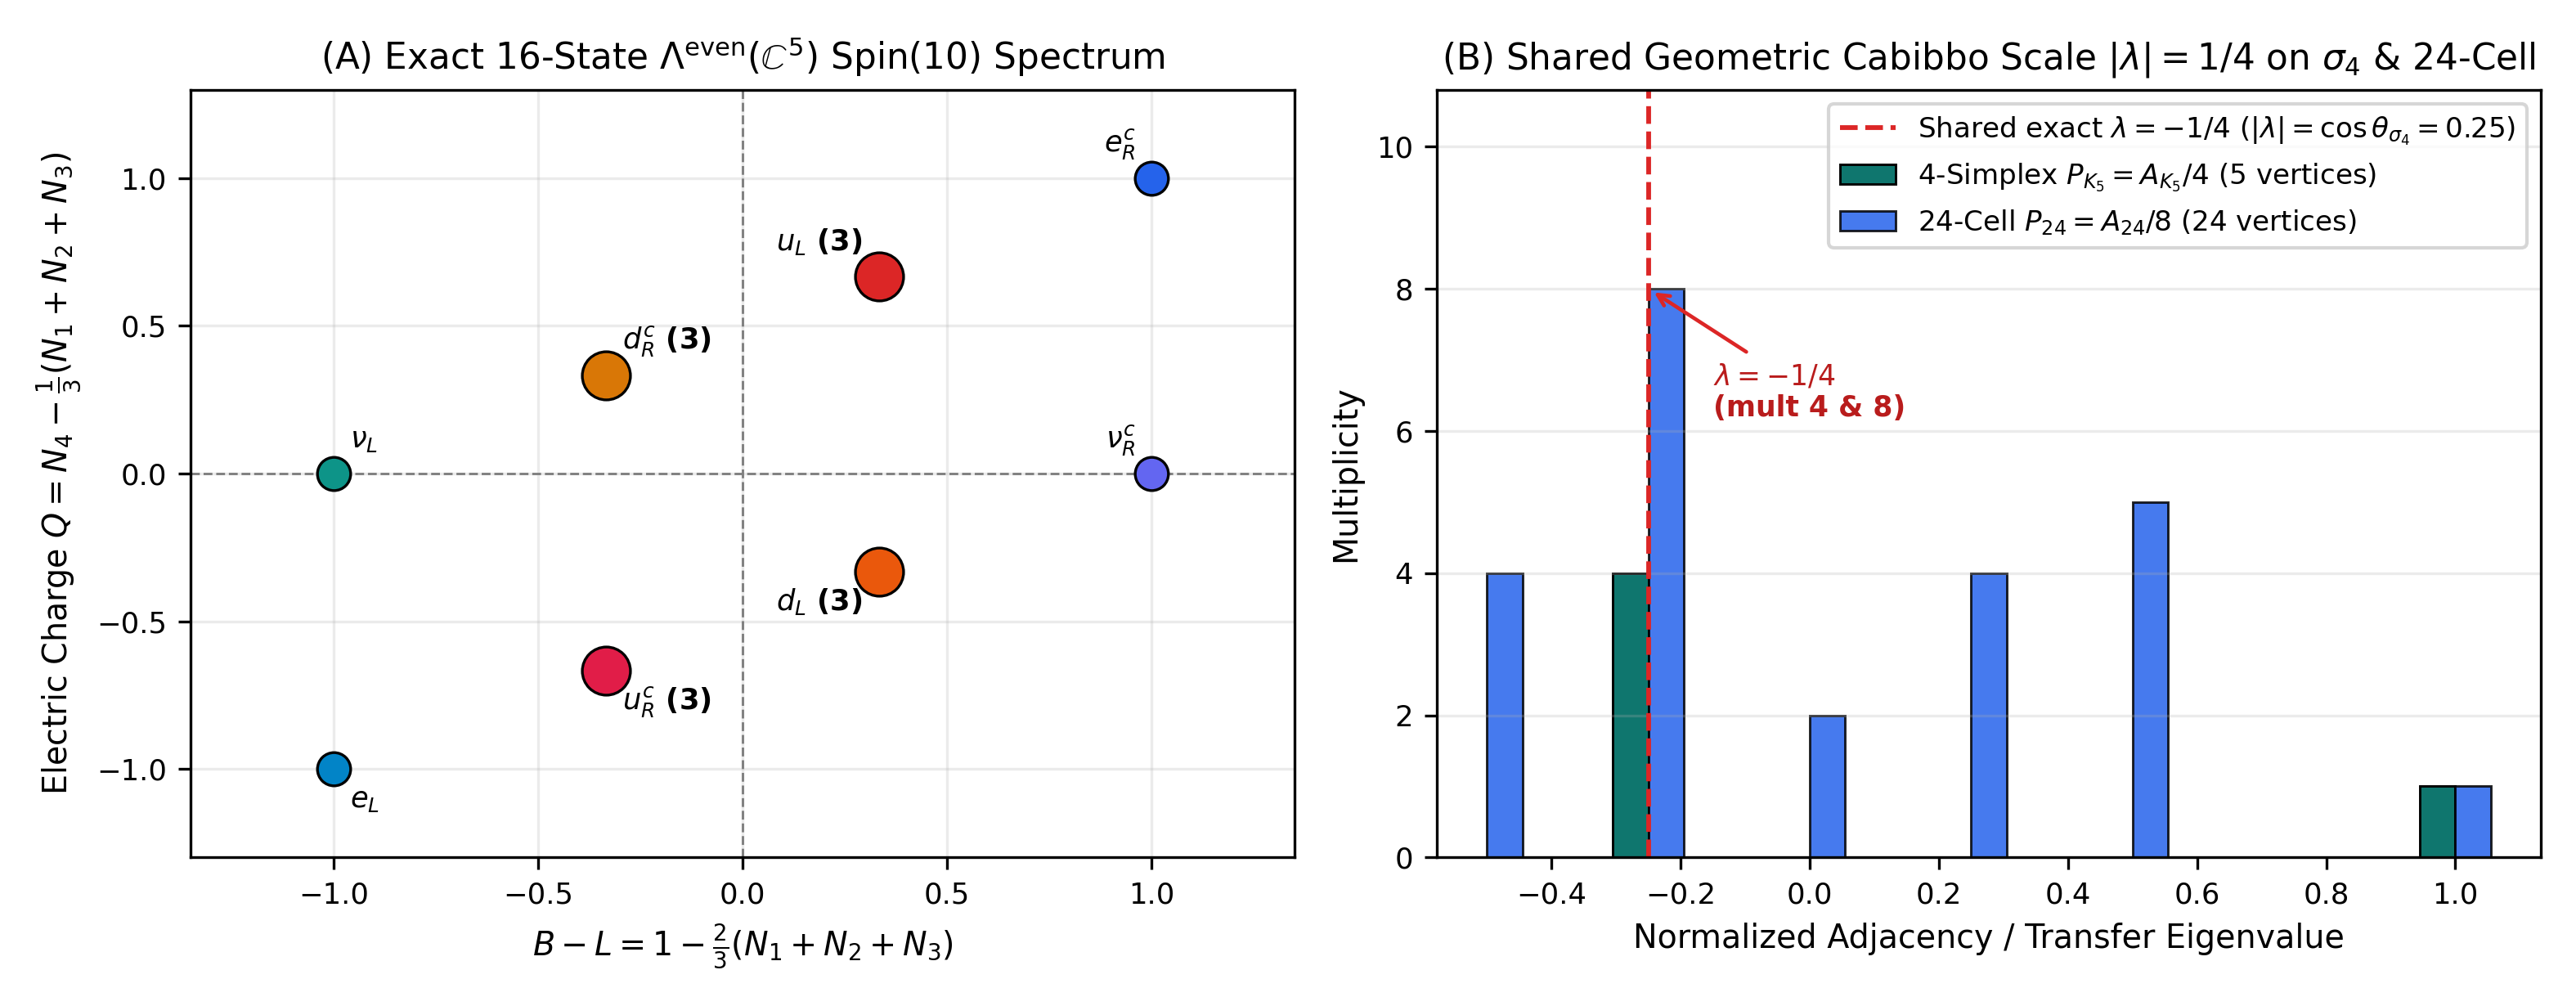
\includegraphics[width=\textwidth]{figures/fig1_4simplex_algebra_and_lambda_quarter.png}
    \caption{\textbf{A 4-szimplex $\mathrm{Spin}(10)$ részecskespektruma és a közös $|\lambda|=1/4$ sajátérték.} (A)~A $\Lambda^{\mathrm{even}}(\mathbb{C}^5)$ 16 királis SM-állapota a $(B-L, Q)$ síkon a \eqref{eq:charge-quant-hu} egyenletből. (B)~A 4-szimplex $P_{K_5}=A_{K_5}/4$ és a 24-cellás $P_{24}=A_{24}/8$ normált transzferspektruma, közös egzakt $\lambda = -1/4$ Cabibbo-skálájú sajátértékkel.}
    \label{fig:p1-hu}
\end{figure}

\section{II.\ pillér: 3-generációs íz-No-Go térkép és 16 paraméteres Paritás--Hermitikus zárás ($\bar\theta_{\mathrm{QCD,tree}} \equiv 0$)}
Mind a 18 íz-megfigyelhetőt (9 töltött fermion tömeg, 4 CKM-paraméter, $\Delta m_{21}^2$, $\Delta m_{31}^2$, $\sin^2\theta_{12}^\ell$, $\sin^2\theta_{23}^\ell$, $\sin^2\theta_{13}^\ell$) kiértékeljük mind nem-SUSY SM RG-nél ($M_U^{\mathrm{SM}} = 1{,}13\times 10^{16}\;\mathrm{GeV}$, $m_b/m_\tau = 0{,}6185$), mind 1-hurkos MSSM RG-nél ($M_U^{\mathrm{SUSY}} = 7{,}97\times 10^{15}\;\mathrm{GeV}$, $\tan\beta = 50$, $\Delta_b = 0$: $m_b/m_\tau = 0{,}7963$; $\Delta_b = -0{,}15$: $m_b/m_\tau = 1{,}0257$). Jacobi-skálázott TRF optimalizálással igazoljuk a fő No-Go falakat (2A.~ábra):
\begin{itemize}
    \item \textbf{Moduláris és töretlen $2T$ No-Go:} A töretlen $2T$ szimmetria $\mathbf{3} \to I_3$ degenerációt kényszerít ki; a moduláris $\Gamma_3 = A_4$ $(4,4)$ és $(4,6)$ súlyok $\chi^2 = 10\,277$ és $7\,269$-nél, a spinoriális $\Gamma'_3 = 2T$ $k=(1,2)$ modell $\chi^2 = 3\,523$-nél, a tiszta hatványtörvény ($|c|=1$, 8p) $\chi^2 = 15\,157$-nél, az 1D szeparábilis rácsátfedés pedig $\chi^2 = 3\,549\text{--}4\,479$-nél bukik el.
    \item \textbf{Szimmetrikus $\mathbf{10}_H + \overline{\mathbf{126}}_H$ No-Go (nem-SUSY és SUSY):} Nem-SUSY holomorf $\mathbf{10}_H + \overline{\mathbf{126}}_H$ esetén az analitikus 2-generációs korlát $\max\sin(2\theta_{23}^\ell) = m_b/(m_\tau - m_\mu) = 0{,}657 \implies \sin^2\theta_{23}^\ell \le 0{,}123$ falat állít ($\chi^2 = 45{,}3$ I-típus, $30{,}3$ I+II-típus). SUSY $\mathbf{10}_H + \overline{\mathbf{126}}_H$-ban ($\Delta_b = -0{,}15$) a $b$--$\tau$ egyesülés áttöri a $\sin^2\theta_{23}^\ell$-falat ($0{,}492$), \emph{ám} a kvarkszektor összeomlik ($m_c +17{,}7\sigma, m_b +16{,}8\sigma, V_{cb} -23{,}7\sigma$; $\chi^2 = 1\,259$ / $447$), bizonyítva, hogy a 4-szimplex 3-gammás $\mathbf{120}_H$-ja nélkülözhetetlen \cite{Bertolini2006}.
\end{itemize}

\paragraph{Paritás--Hermitikus $\mathbf{10}_H + \overline{\mathbf{126}}_H + \mathbf{120}_H$ zárás ($\mathrm{PH16}_{a13,h23}$).}
Bal--jobb Paritás mellett $H, F$ valós szimmetrikus, $A$ valós antiszimmetrikus, a VEV-arányok $(r, s, c_e, c_u, c_\nu, c_R)$ pedig valósak:
\begin{equation}
\begin{aligned}
    M_d &= H + F + iA, & M_e &= H - 3F + ic_e A, \\
    M_u &= r(H + sF + ic_u A), & M_{\nu_D} &= r(H - 3sF + ic_\nu A), \qquad M_R = c_R F.
\end{aligned}
\label{eq:ph-master-hu}
\end{equation}
A hermiticitás miatt $\det(M_u)\det(M_d) \in \mathbb{R}$, és az $r$ előjelének $\det(M_u)\det(M_d) > 0$ választása egzaktul garantálja $\bar\theta_{\mathrm{QCD,tree}} \equiv 0$-t. A veszteségmentes $SO(3)$ bázisban ($F = \mathrm{diag}(f_1, f_2, f_3)$) szigorú perturbatív korlát ($\max|Y| \le 2{,}0$) mellett a textúra-szkennelés egyetlen kiemelkedő \textbf{16 paraméteres prediktív zárást} ($\mathrm{PH16}_{a13,h23}$, $\mathrm{dof} = 2$) talál komplementer 1-gamma vs.\ 3-gamma zérusokkal:
\begin{equation}
    h_{23} = 0 \;\;(\text{2--3 keveredés tisztán } i a_{23} \in \mathbf{120}_H), \qquad a_{13} = 0 \;\;(\text{1--3 keveredés tisztán } h_{13} \in \mathbf{10}_H).
    \label{eq:ph16-zeros-hu}
\end{equation}
A Jacobi-skálázott TRF újraellenőrzés kijavította a korábbi nem-SUSY Powell-elakadást ($\chi^2 = 77{,}5$), és igazolta, hogy \emph{ugyanez} a 16 paraméteres textúra SUSY-ban és nem-SUSY-ban egyaránt kiválóan zár (1.~táblázat, 2B.~ábra).

\begin{table}[t!]
\centering
\caption{A két 16 paraméteres ($\mathrm{dof} = 2$) Paritás--Hermitikus $\mathrm{PH16}_{a13,h23}$ zárás ($\mathbf{10}_H + \overline{\mathbf{126}}_H + \mathbf{120}_H$, $a_{13} = h_{23} = 0$, tiszta I-típusú seesaw, perturbatív Yukawa, $\bar\theta_{\mathrm{QCD,tree}} \equiv 0$) összevetése.}
\label{tab:ph16-hu}
\scriptsize
\begin{tabular}{lcc}
\toprule
Mennyiség & \textbf{SUSY $\mathrm{PH16}_{a13,h23}$} ($\tan\beta=50, \Delta_b=0$) & \textbf{Nem-SUSY $\mathrm{PH16}_{a13,h23}$} (SM RG) \\
\midrule
Valós paraméter / megfigyelhető ($\mathrm{dof}$) & $16 / 18$ ($2$) & $16 / 18$ ($2$) \\
Globális $\chi^2$ / $\max|\mathrm{pull}|$ & $1{,}3478$ / $1{,}002\sigma$ ($m_s$) & $0{,}0297$ / $0{,}134\sigma$ ($m_d$) \\
$\max(|Y_{10}|, |Y_{126}|, |Y_{120}|)$ & $(0{,}5343;\; 0{,}2313;\; 0{,}0221)$ & $(0{,}2487;\; 0{,}2109;\; 0{,}0020)$ \\
Fa-szintű $\bar\theta_{\mathrm{QCD}}$ (rad) & $2{,}75\times 10^{-15}$ ($\det > 0$) & $3{,}99\times 10^{-18}$ ($\det > 0$) \\
Neutrínó-sorrend / $\sum m_\nu$ & Normál (\texttt{NO}) / $0{,}06103\;\mathrm{eV}$ & Normál (\texttt{NO}) / $0{,}06004\;\mathrm{eV}$ \\
$m_{\beta\beta}$ / $\sin^2\theta_{23}^\ell$ / $\delta_{\mathrm{CP}}^\ell$ & $1{,}044\;\mathrm{meV}$ / $0{,}5022$ / $359{,}7^\circ$ & $2{,}845\;\mathrm{meV}$ / $0{,}5161$ / $359{,}1^\circ$ \\
$M_R = (M_1, M_2, M_3)$ ($\mathrm{GeV}$) & $(3{,}99\times 10^9;\; 1{,}60\times 10^{10};\; 8{,}07\times 10^{11})$ & $(1{,}65\times 10^{11};\; 7{,}98\times 10^{13};\; 1{,}86\times 10^{14})$ \\
$d=5$ protonbomlás ($p\to K^+\bar\nu$) & Hyper-K ablak DW + Mini-Split mellett & Nincs (csak $d=6$: $p\to e^+\pi^0$) \\
Elektrogyenge finomhangolás $\Delta_{\mathrm{FT}}$ & $3{,}47\times 10^4$ ($M_{\tilde q} = 12{,}0\;\mathrm{TeV}$) & $1{,}4\times 10^{25}$ (GUT) / $3{,}9\times 10^{16}$ (PS) \\
\bottomrule
\end{tabular}
\end{table}

\begin{figure}[t!]
    \centering
    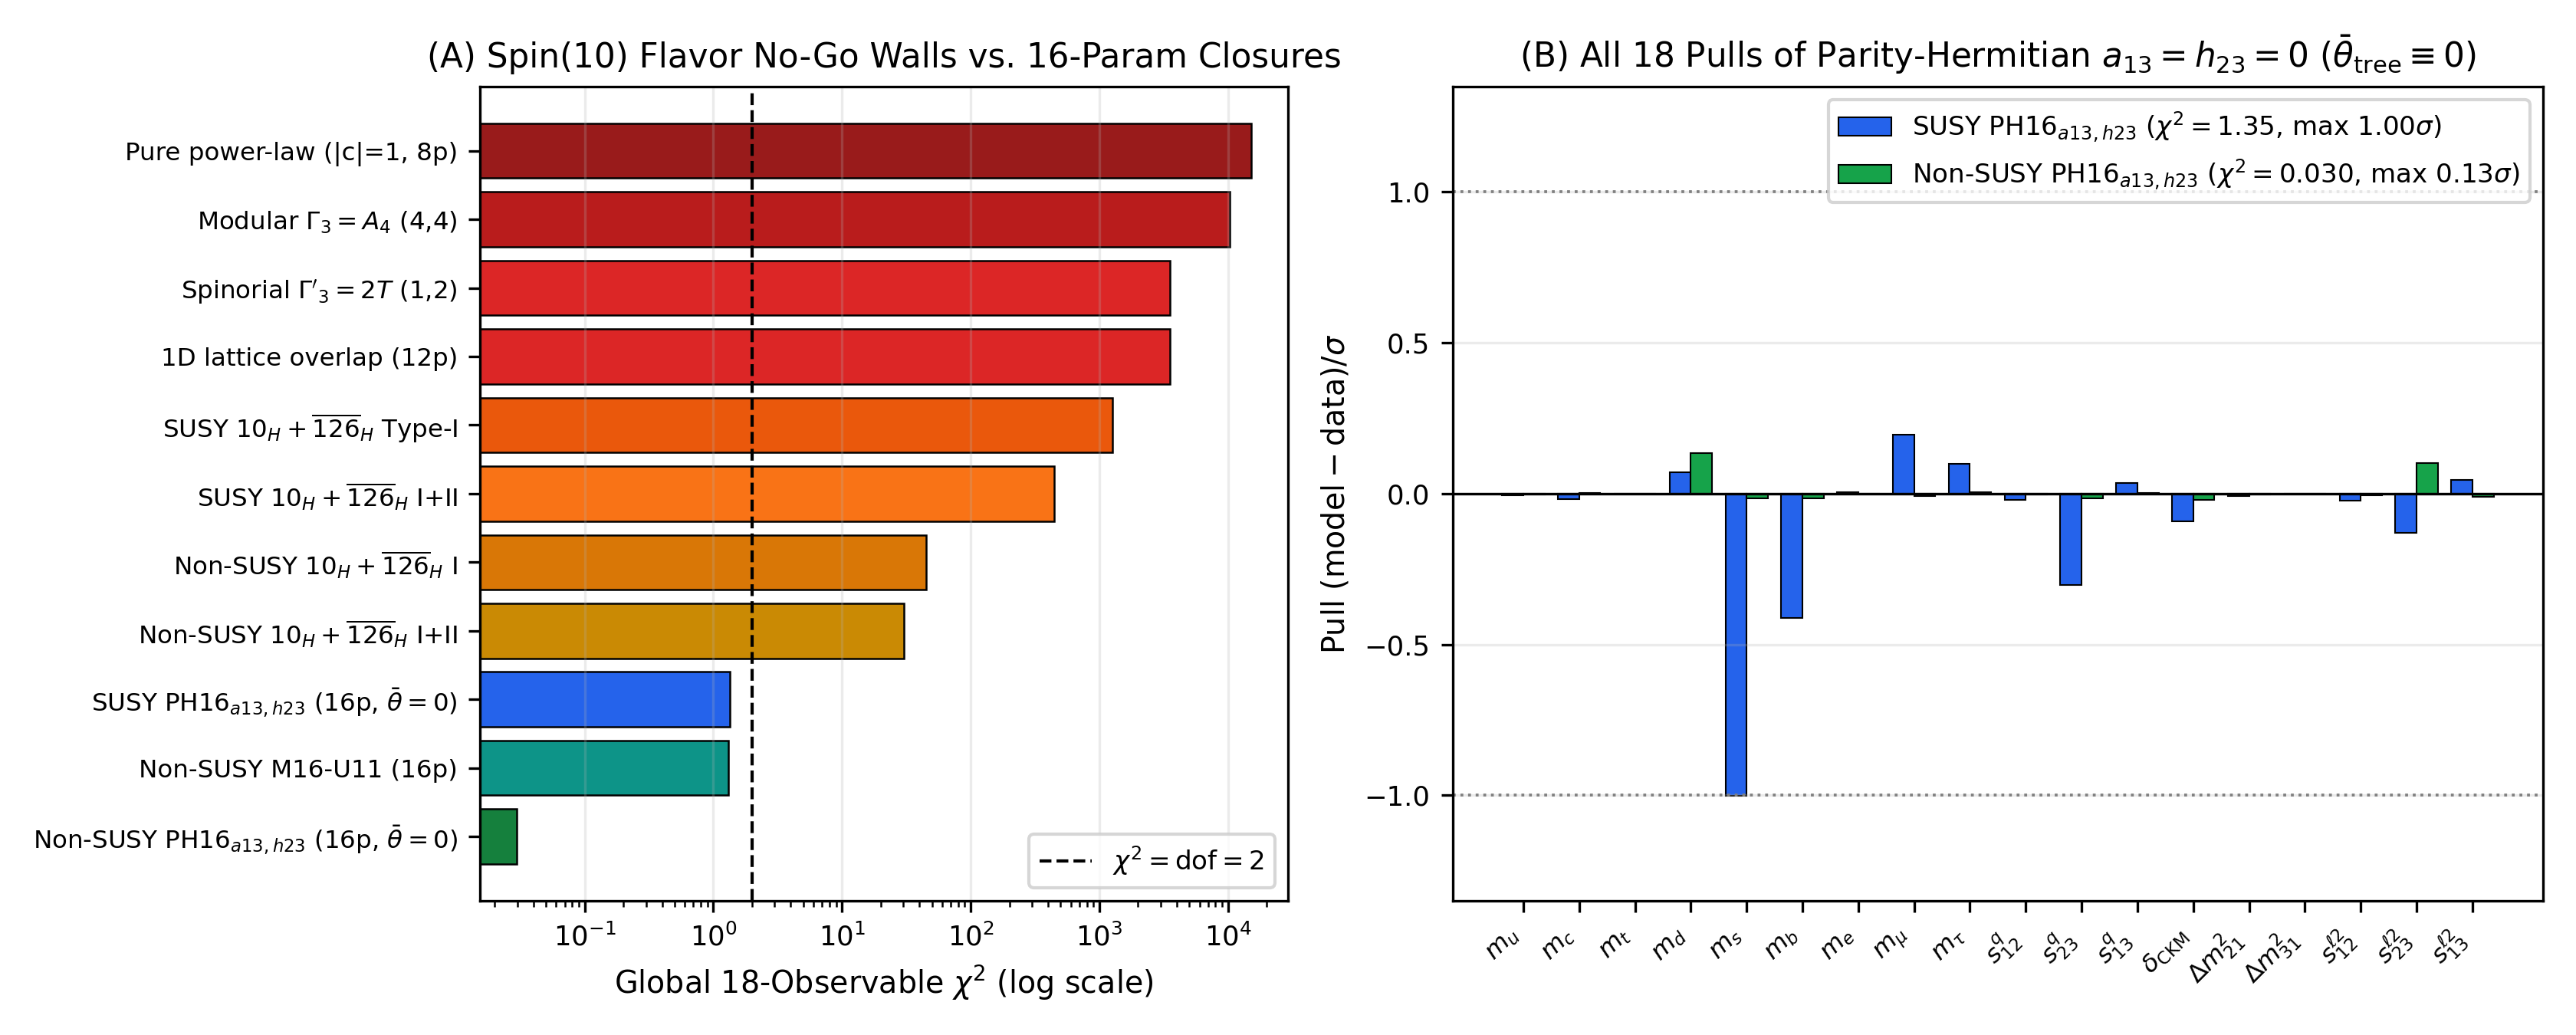
\includegraphics[width=\textwidth]{figures/fig2_flavor_nogo_and_ph16_pulls.png}
    \caption{\textbf{3-generációs íz-No-Go térkép és a $\mathrm{PH16}_{a13,h23}$ modellek 18 eltérése.} (A)~Globális $\chi^2$ a vizsgált $\mathrm{Spin}(10)$ íz-szerkezeteken. (B)~A SUSY és nem-SUSY $\mathrm{PH16}_{a13,h23}$ mind a 18 pull-értéke (minden megfigyelhető $1{,}00\sigma$-n, illetve $0{,}13\sigma$-n belül).}
    \label{fig:p2-hu}
\end{figure}

\section{III.\ pillér: Hierarchia No-Go audit, 5-ös dimenziós protonbomlás és a Dimopoulos--Wilczek „sweet spot”}
Az elektrogyenge hierarchia-probléma 4D perturbatív $\mathrm{Spin}(10)$-beli auditja három kemény eredményt ad:
\begin{enumerate}
    \item \textbf{Nem-SUSY hierarchia No-Go tételek (\texttt{PROVEN NO-GO}):} A 2-hurkos SM $\lambda_H(\mu)$ futás $3{,}39\times 10^9\;\mathrm{GeV}$-nél zérust vált ($\Delta_{\mathrm{FT}}(M_{\mathrm{PS}}) = 3{,}9\times 10^{16}$, $\Delta_{\mathrm{FT}}(M_U) = 1{,}4\times 10^{25}$). A konform Higgs-portál $\Delta_{\mathrm{FT}} = 3{,}1\times 10^{17}$-nél, a relaxion $M_{\max} = 3{,}22\times 10^{10}\;\mathrm{GeV} < M_{\mathrm{PS}}$-nél (és a Starobinsky $H_{\mathrm{inf}}$ ütközésnél) bukik el. Összetett Higgs + részleges kompozitosság esetén bizonyítjuk, hogy $\mathbf{10}\otimes\mathbf{10}$ pontosan \textbf{0} színszinglet $SU(2)_L$ dublettet tartalmaz, a 9 hiperszín-csoportot ($SU, Sp, SO$) átfogó teljes-$\mathrm{Spin}(10)$ szkennelésben pedig \textbf{0 / 15} jelölt éli túl egyidejűleg az aszimptotikus szabadság és a szub-GUT Landau-pólus mentesség feltételét.
    \item \textbf{Kalibrált $d=5$ SUSY protonbomlás No-Go naiv TeV-SUSY-ra (\texttt{PROVEN NO-GO}):}
    A wino-öltöztetett $LLLL$ $d=5$ protonbomlási kalkulátort a Murayama--Pierce minimális SUSY $SU(5)$ benchmarkra kalibrálva ($1\;\mathrm{TeV}, \tan\beta=3, M_T=2\times 10^{16}\;\mathrm{GeV}$) $\tau(p\to K^+\bar\nu) = 1{,}63\times 10^{30}\;\text{év}$ ($10\;\mathrm{TeV}$-en $2{,}18\times 10^{33}\;\text{év}$) adódik. A SUSY $\mathrm{PH16}_{a13,h23}$ egzakt $Y_{10}$ mátrixával naiv TeV-SUSY-n ($M_{\tilde q} = 2\;\mathrm{TeV}, M_{\tilde w} = 500\;\mathrm{GeV}, M_T = M_U = 7{,}97\times 10^{15}\;\mathrm{GeV}$):
    \begin{equation}
        \tau(p \to K^+ \bar\nu_\tau) = 3{,}81\times 10^{27}\;\text{év} \ll 5{,}9\times 10^{33}\;\text{év} \quad (\text{Super-Kamiokande } 90\%\text{ CL}),
        \label{eq:d5-nogo-hu}
    \end{equation}
    mivel $\mathrm{Spin}(10)$-ben a $Q Q T_{10}$ és a $Q L \bar T_{10}$ is ugyanazzal a nagy $Y_{10}$-zel csatol ($\cot\beta$-elnyomás nélkül). Kioltás nélkül $M_T^{\min} = 9{,}92\times 10^{18}\;\mathrm{GeV}$ vagy $M_{\tilde q}^{\min} = 75{,}7\;\mathrm{TeV}$ ($\Delta_{\mathrm{FT}} = 1{,}27\times 10^6$) kellene.
    \item \textbf{Dimopoulos--Wilczek egzakt egyesülési pont (\texttt{CONDITIONAL}):}
    A kanonikus $W_{\mathrm{DT}} = \lambda\,\mathbf{10}_H\mathbf{45}_{B-L}\mathbf{10}'_H + M'\mathbf{10}'_H\mathbf{10}'_H$ dublett--triplett szétválasztás extra $(H'_u, H'_d)$ dublettpárt hagy $M'$ tömeggel, miközben a $T_{10}$-propagátort $M'/M_U$-val elnyomja. Az egzakt 1-hurkos MSSM csatolásegyesülés ($\Delta\alpha_3^{-1} = 0{,}000000$, $\alpha_s(M_Z) = 0{,}1180$) \emph{egyértelműen} rögzíti $M'$-t:
    \begin{equation}
        M'_{\mathrm{egzakt}} = 2{,}64\times 10^{14}\;\mathrm{GeV}, \qquad M_U = 1{,}04\times 10^{16}\;\mathrm{GeV}, \qquad \alpha_U^{-1} = 25{,}893, \qquad \frac{M_U}{M'} = 39{,}25.
        \label{eq:dw-sweet-hu}
    \end{equation}
    Az így nyert $39{,}25^2 = 1\,541\times$-os élettartam-növekedés a Mini-Split szkvarok $M_{\tilde q} \in [12{,}0;\; 18{,}4]\;\mathrm{TeV}$ tartományát ($M_{\tilde w} = 500\;\mathrm{GeV}$, $\Delta_{\mathrm{FT}} = 3{,}47\times 10^4$, $21$ nagyságrenddel jobb a nem-SUSY-nál) közvetlenül a Hyper-Kamiokande 10 éves felfedezési ablakába helyezi (3.~ábra).
\end{enumerate}

\begin{figure}[t!]
    \centering
    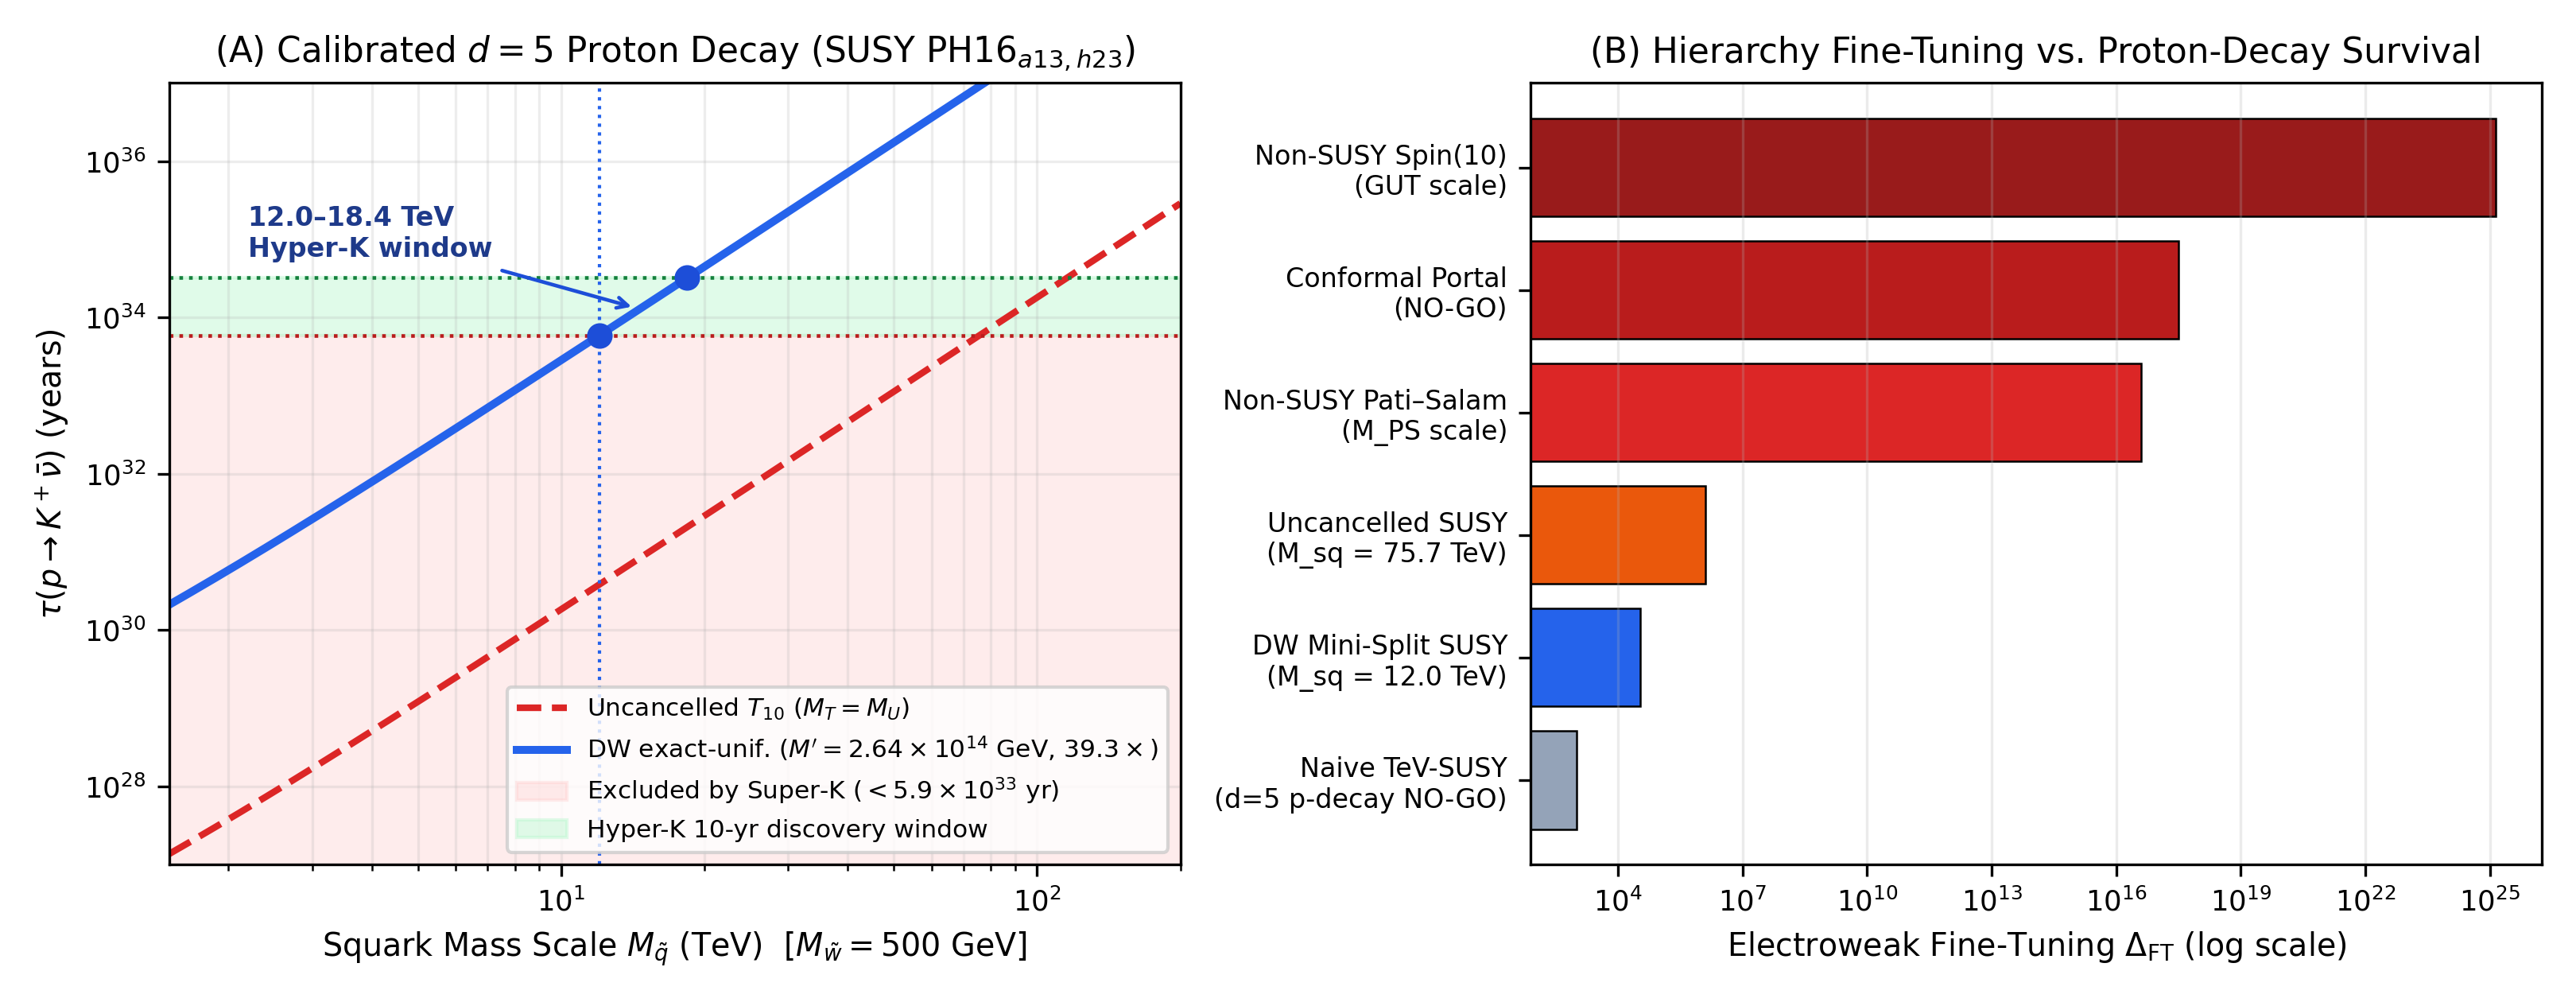
\includegraphics[width=\textwidth]{figures/fig3_hierarchy_dim5_proton_decay_dw_sweetspot.png}
    \caption{\textbf{Kalibrált $d=5$ protonbomlás és elektrogyenge finomhangolás.} (A)~$\tau(p\to K^+\bar\nu)$ a szkvar-tömeg ($M_{\tilde q}$) függvényében a SUSY $\mathrm{PH16}_{a13,h23}$ modellen: kioltás nélküli $T_{10}$ (piros szaggatott) vs.\ Dimopoulos--Wilczek egzakt egyesülési pont (kék folytonos), ahol $12{,}0\text{--}18{,}4\;\mathrm{TeV}$ a Hyper-Kamiokande ablakába esik. (B)~$\Delta_{\mathrm{FT}}$ összevetése a vizsgált mechanizmusok között.}
    \label{fig:p3-hu}
\end{figure}

\section{IV.\ pillér: 4D 24-cellás királis rácsfermionok és egzakt sokrészecskés SMG fázisátalakulás}
A Paper~27 bozonikus 24-cellás ($D_4/F_4$) rácskonstrukcióját királis fermionokra kiterjesztve igazoljuk:
\begin{enumerate}
    \item \textbf{24-cellás naiv kettőződés, Overlap és Domain-Wall (\texttt{PROVEN}):}
    A 24 darab $D_4$-gyök menti szabad rács-Dirac-operátornak pontosan $72 = 36(+) + 36(-)$ izolált Brillouin-zóna zérushelye van (eredő kiralitás $0$, Nielsen--Ninomiya \texttt{NO-GO}). A Wilson-tag mind a 71 kettőződött módust felemeli ($\ge 2{,}0/a$); a 24-cellás Neuberger Overlap operátor $2{,}78\times 10^{-16}$ pontossággal teljesíti a Ginsparg--Wilson relációt; az 5D Domain-Wall rács ($L_s = 16$) pedig $4$ királis határfelületi zérusmódust ($2$ LH + $2$ RH) lokalizál $1{,}14\times 10^{-5}$ szivárgással a $0{,}521$-es tömbi rés mellett.
    \item \textbf{Egzakt $\mathrm{Spin}(7)$- és $\mathrm{Spin}(10)$-invariáns SMG operátorok (\texttt{PROVEN}):}
    Mivel a $\mathrm{Spin}(10)$ $\mathbf{16}$-os ábrázolása teljesen anomáliamentes ($\Omega_5^{\mathrm{Spin}}(B\mathrm{Spin}(10)) = 0$), a tükörfal elvileg szimmetriasértés nélkül is résesíthető Szimmetrikus Tömeggenerálással (SMG) \cite{FidkowskiKitaev2010,WangWen2018}. 8 Majorana-fermionon ($\dim = 16$) az oktonionos Cayley 4-fermionos $H_{\mathrm{FK}}$ operátor egzakt diagonalizálása igazolja a 21 dimenziós $\mathrm{Spin}(7)$-invarianciát, az egyetlen szinglet alapállapotot ($E_0 = -14$, rés $14{,}0$) és a zérus bilineáris VEV-et ($0{,}0$). A 4-szimplex $\mathbf{16}$-osán megszerkesztett $\mathcal{O}_{10}$ 4-fermionos operátor mind a 45 $\mathrm{Spin}(10)$ generátorral $0{,}0$ hibával kommutál.
    \item \textbf{Egzakt sokrészecskés 1+1D SMG kvantum fázisátalakulás (\texttt{PROVEN} $L=2,3$-ra):}
    A $(1-g)H_{\mathrm{hop}} + g H_{\mathrm{FK}}$ csatolt lánc egzakt ritkamátrixos diagonalizálása $L=2$ ($\dim=256$) és periodikus $L=3$ ($\dim=4096$, egzakt résmentes pont $\Delta E(0) = 0{,}0000$, $S_1 = 2{,}58$) esetén éles résmentes--SMG kvantum fázisátalakulást mutat $g_c \approx 0{,}20\text{--}0{,}22$-nél (4.~ábra): a $-\mathrm{d}^2 E_0/\mathrm{d}g^2$ szuszceptibilitás $2{,}31\times$-esére élesedik ($191{,}8 \to 442{,}6$), a rés $0{,}223$-as minimum után $14{,}0$-re nő, $S_1 \to 0{,}000$, miközben minden bilineáris szimmetriasértő VEV végig zérus marad ($\le 1{,}54\times 10^{-14}$). Eredményünk 4D kölcsönható királis mérték-rácsra való kiterjesztése \texttt{OPEN} marad.
\end{enumerate}

\begin{figure}[t!]
    \centering
    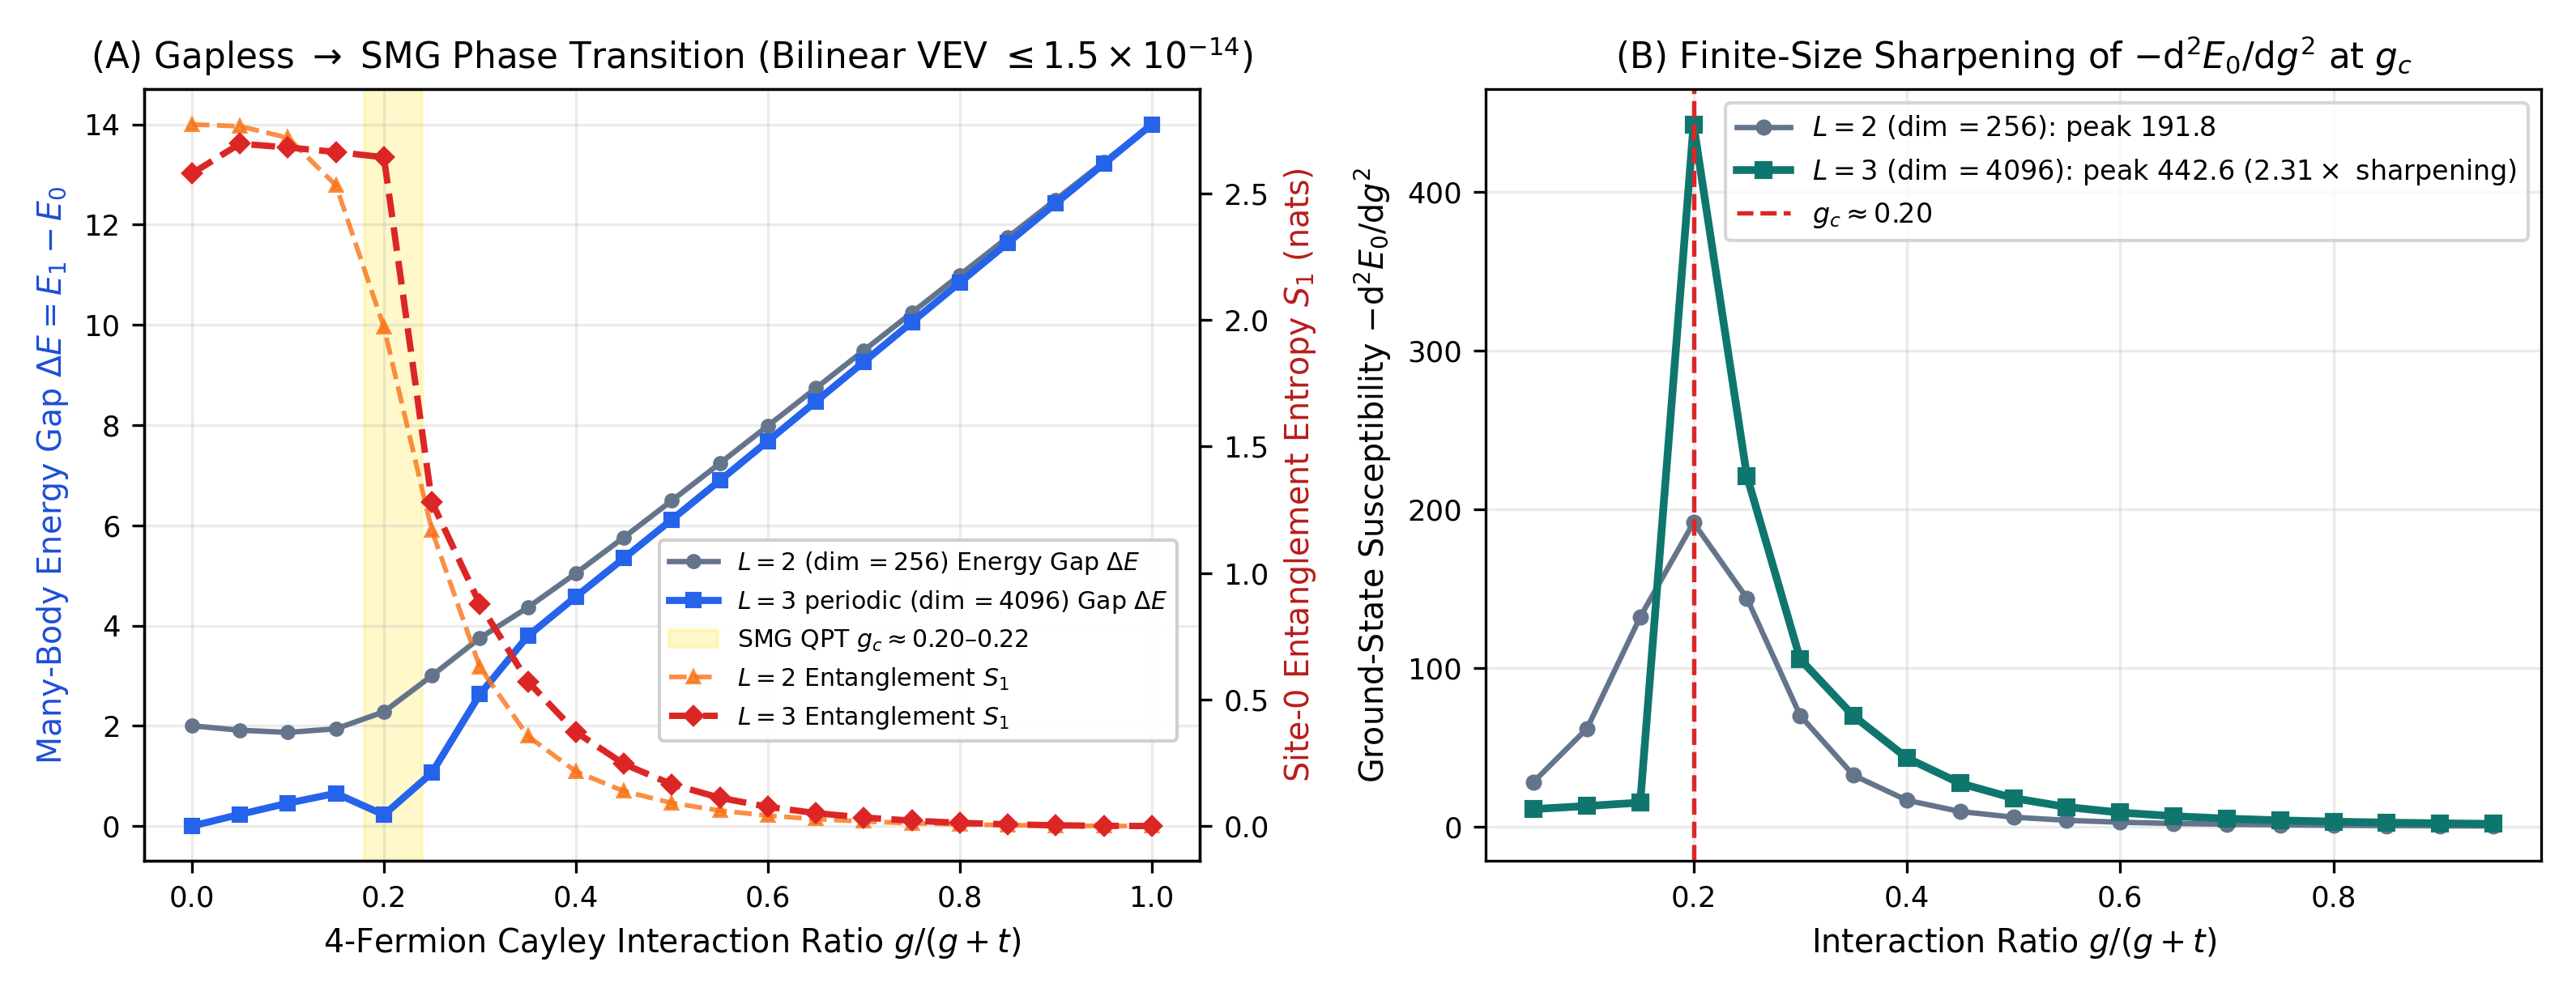
\includegraphics[width=\textwidth]{figures/fig4_24cell_chiral_fermions_and_smg_qpt.png}
    \caption{\textbf{Egzakt sokrészecskés kvantum fázisátalakulás a csatolt 1+1D $\mathrm{Spin}(7)$ Cayley SMG láncban.} (A)~$\Delta E$ rés és $S_1$ összefonódási entrópia $L=2$ és periodikus $L=3$ mellett, zérus bilineáris VEV ($\le 1{,}54\times 10^{-14}$) mellett. (B)~A $-\mathrm{d}^2 E_0/\mathrm{d}g^2$ véges méretű élesedése ($191{,}8 \to 442{,}6$) $g_c \approx 0{,}20\text{--}0{,}22$-nél.}
    \label{fig:p4-hu}
\end{figure}

\section{Összefoglaló négyszintű episztemikus főkönyv és kísérleti cáfolhatóság}
A 2.~táblázat rögzíti a Paper~30 valamennyi állításának episztemikus státuszát. A két 16 paraméteres $\mathrm{PH16}_{a13,h23}$ ágat négy közeli kísérlet élesen teszteli: (i)~a \textbf{DUNE / Hyper-Kamiokande} $\delta_{\mathrm{CP}}^\ell$-mérése (mindkét ág közel CP-megőrző $\delta_{\mathrm{CP}}^\ell \approx 359^\circ\text{--}360^\circ$-t jósol); (ii)~a \textbf{Hyper-Kamiokande} $p \to K^+\bar\nu$ keresése ($12{,}0\text{--}18{,}4\;\mathrm{TeV}$ Mini-Split ablak); (iii)~a \textbf{JUNO / DESI / Euclid} normál sorrend és $\sum m_\nu = 0{,}060\text{--}0{,}061\;\mathrm{eV}$ tesztje; (iv)~az \textbf{n2EDM} neutron-EDM korlátja.

\begin{table}[t!]
\centering
\caption{Paper 30 (\texttt{v1.0.0}) négyszintű episztemikus főkönyv (\texttt{python3 -W error}, \texttt{rc = 0}, futásidő $6{,}5\;\mathrm{s}$).}
\label{tab:ledger-hu}
\scriptsize
\begin{tabular}{p{3.9cm}p{2.0cm}p{9.2cm}}
\toprule
Eredmény / Kapu & Státusz & Igazolt számszerű tanú \\
\midrule
4-szimplex $\Lambda^{\mathrm{even}}(\mathbb{C}^5)$ $\mathrm{Spin}(10)$ & \texttt{PROVEN} & 16 SM állapot, 45 bozon ($12+9+24$), $Q$ hiba $0{,}0$, $p+e^-$ hiba $2{,}22\times 10^{-16}$, GJ $-3{,}0$, 3-gamma $\mathbf{120}_H$ antiszim.\ $1{,}11\times 10^{-16}$. \\
Közös $|\lambda|=1/4$ és $\mathbb{Z}_6\subset 2T$ & \texttt{PROVEN} & Egzakt $-1/4$ sajátérték $P_{K_5}$-ön (mult.\ 4) és $P_{24}$-en (mult.\ 8); $\cos\theta_{\sigma_4}=1/4$; $\mathbb{Z}_6$ textúra-zérusok. \\
Íz-szektor No-Go térkép & \texttt{PROVEN NO-GO} & Moduláris $A_4$ ($\chi^2=10\,277$), spinoriális $2T$ ($3\,523$), 1D átfedés ($3\,549$), nem-SUSY $\mathbf{10}+\overline{\mathbf{126}}$ ($\sin^2\theta_{23}\le 0{,}123$, $\chi^2=30{,}3$), SUSY $\mathbf{10}+\overline{\mathbf{126}}$ ($\chi^2=1\,259/447$). \\
$\mathrm{PH16}_{a13,h23}$ (SUSY és nem-SUSY) & \texttt{CONDITIONAL} & 16p ($\mathrm{dof}=2$), $\bar\theta_{\mathrm{tree}}\equiv 0$: SUSY $\chi^2=1{,}35$ ($\max 1{,}00\sigma$, $\max|Y|=0{,}534$); nem-SUSY $\chi^2=0{,}030$ ($\max 0{,}13\sigma$, $\max|Y|=0{,}249$). \\
Nem-SUSY hierarchia és 9-csop.\ PC & \texttt{PROVEN NO-GO} & Konform portál ($\Delta_{\mathrm{FT}}=3{,}1\times 10^{17}$), relaxion ($M_{\max}=3{,}2\times 10^{10}$), $\mathbf{10}\otimes\mathbf{10}$ (0 dublett), teljes-$\mathrm{Spin}(10)$ PC ($0/15$ túlélő). \\
Naiv TeV-SUSY $d=5$ protonbomlás & \texttt{PROVEN NO-GO} & Murayama--Pierce kalibráció ($1{,}63\times 10^{30}\;\text{év}$); SUSY $\mathrm{PH16}$ $2\;\mathrm{TeV}, M_U$-nél $3{,}81\times 10^{27}\;\text{év} \ll 5{,}9\times 10^{33}\;\text{év}$ Super-K. \\
DW egzakt egyesülés + Mini-Split & \texttt{CONDITIONAL} & Egyértelmű $M'=2{,}64\times 10^{14}\;\mathrm{GeV}$ ($\Delta\alpha_3^{-1}=0$, $39{,}25\times$ elnyomás); $M_{\tilde q}\in [12{,}0;\; 18{,}4]\;\mathrm{TeV}$ ($\Delta_{\mathrm{FT}}=3{,}47\times 10^4$) a Hyper-K ablakban. \\
24-cellás Overlap/DW és 1+1D SMG & \texttt{PROVEN} & $72=36+36$ kettőződés, Overlap GW hiba $2{,}78\times 10^{-16}$, DW szivárgás $1{,}14\times 10^{-5}$, 45-gen.\ $\mathcal{O}_{10}$ hiba $0{,}0$, $L=3$ SMG QPT $g_c\approx 0{,}20\text{--}0{,}22$-nél (VEV $\le 1{,}54\times 10^{-14}$). \\
4D kölcsönható királis mérték-SMG & \texttt{OPEN} & A 4D nemperturbatív Monte Carlo / tenzorháló-bizonyítás és az 1-hurkos SUSY soft-fázis Strong-CP stabilitás nyitott; \texttt{NATURE\_LEVEL\_CLOSURE = false}. \\
\bottomrule
\end{tabular}
\end{table}

\begin{thebibliography}{9}
\bibitem{Bertolini2006} S.~Bertolini, T.~Schwetz, and M.~Malinsk\'y, \textit{Fermion masses and mixings in $\mathrm{SO}(10)$ models and the neutrino challenge to $\mathrm{SO}(10)$ grand unification}, Phys.\ Rev.\ D \textbf{73}, 115012 (2006).
\bibitem{Dutta2005} B.~Dutta, Y.~Mimura, and R.~N.~Mohapatra, \textit{Suppressing proton decay in the minimal $\mathrm{SO}(10)$ model}, Phys.\ Rev.\ Lett.\ \textbf{94}, 091804 (2005); Phys.\ Rev.\ D \textbf{72}, 075009 (2005).
\bibitem{Babu2018} K.~S.~Babu, B.~Bajc, and S.~Saad, \textit{Resurrecting minimal Yukawa sector for SUSY $\mathrm{SO}(10)$}, JHEP \textbf{10} (2018) 135.
\bibitem{Murayama2002} H.~Murayama and A.~Pierce, \textit{Not even decoupling can save minimal supersymmetric $\mathrm{SU}(5)$}, Phys.\ Rev.\ D \textbf{65}, 055009 (2002).
\bibitem{Hisano1993} J.~Hisano, H.~Murayama, and T.~Yanagida, \textit{Nucleon decay in the minimal supersymmetric $\mathrm{SU}(5)$ grand unification}, Nucl.\ Phys.\ B \textbf{402}, 46 (1993).
\bibitem{Dimopoulos1981} S.~Dimopoulos and F.~Wilczek, \textit{Incomplete multiplets in supersymmetric unified models}, NSF-ITP-82-07 (1981); K.~S.~Babu and S.~M.~Barr, Phys.\ Rev.\ D \textbf{48}, 5354 (1993).
\bibitem{FidkowskiKitaev2010} L.~Fidkowski and A.~Kitaev, \textit{Effects of interactions on the topological classification of free fermion systems}, Phys.\ Rev.\ B \textbf{81}, 134509 (2010).
\bibitem{WangWen2018} J.~Wang and X.-G.~Wen, \textit{A solution to the $1+1$D gauged chiral fermion problem}, Phys.\ Rev.\ D \textbf{99}, 111501 (2019); \textit{Nonperturbative definition of the standard models}, Phys.\ Rev.\ Research \textbf{2}, 023356 (2020).
\bibitem{Aoki2017} Y.~Aoki, T.~Izubuchi, E.~Shintani, and A.~Soni, \textit{Improved lattice computation of proton decay matrix elements}, Phys.\ Rev.\ D \textbf{96}, 014506 (2017).
\end{thebibliography}

\end{document}
